\documentclass[10pt]{article}

  \usepackage{pgfplots}
\pgfplotsset{compat=newest}
%% the following commands are needed for some matlab2tikz features
\usetikzlibrary{plotmarks}
\usetikzlibrary{arrows.meta}
\usepgfplotslibrary{patchplots}
\usepackage{grffile}
\usepackage{amsmath}
\usepackage{lineno}


%\usepackage{fullpage}
\usepackage[top=0.0in, bottom=1in, left=0.8in, right=1in]{geometry}
\usepackage{multicol}
\usepackage{caption}
\usepackage{subcaption}
\usepackage{hyperref}
\usepackage{xcolor}
\usepackage{graphicx,psfrag}
\usepackage[pdf]{pstricks}

\definecolor{lightblue}{rgb}{.80,.9,1}
\newcommand{\hl}[1]
    {\par\colorbox{lightblue}{\parbox{\linewidth}{#1}}}

\newcommand{\defn}{\stackrel{\textrm{\scriptsize def}}{=}}

\setlength{\columnsep}{0.1pc}

\title{Non-linear dispersive water wave models}
\author{Jordan Pitt}
\date{}

% TIME ON EVERY PAGE AS WELL AS THE FILE NAME
\usepackage{fancyhdr}
\usepackage{currfile}
\usepackage[us,12hr]{datetime} % `us' makes \today behave as usual in TeX/LaTeX
\pagestyle{plain}

\definecolor{mycolor1}{rgb}{0.00000,0.44700,0.74100}%
\definecolor{mycolor2}{rgb}{0.85000,0.32500,0.09800}%
\definecolor{mycolor3}{rgb}{0.92900,0.69400,0.12500}%
\definecolor{mycolor4}{rgb}{0.49400,0.18400,0.55600}%
\definecolor{mycolor5}{rgb}{0.46600,0.67400,0.18800}% 
\definecolor{mycolor6}{rgb}{0.30100,0.74500,0.93300}%
\definecolor{mycolor7}{rgb}{0.63500,0.07800,0.18400}%

\newcommand\T{\rule{0pt}{3ex }}       % Top table strut
\newcommand\B{\rule[-4ex]{0pt}{4ex }} % Bottom table strut

\newcommand\TM{\rule{0pt}{2.8ex }}       % Top matrix strut
\newcommand\BM{\rule[-2ex]{0pt}{2ex }} % Bottom matrix strut

\newcommand{\vecn}[1]{\boldsymbol{#1}}
\DeclareRobustCommand{\solidrule}[1][0.25cm]{\rule[0.5ex]{#1}{1.5pt}}

\DeclareRobustCommand{\dashedrule}{\mbox{%
		\solidrule[2mm]\hspace{2mm}\solidrule[2mm]}}

\DeclareRobustCommand{\tikzcircle}[1]{\tikz{\filldraw[#1] (0,0) circle (0.5ex);}}	
	
	
\DeclareRobustCommand{\squaret}[1]{\tikz{\draw[#1,thick] (0,0) rectangle (0.2cm,0.2cm);}}
\DeclareRobustCommand{\circlet}[1]{\tikz{\draw[#1,thick] (0,0) circle [radius=0.1cm];}}
\DeclareRobustCommand{\trianglet}[1]{\tikz{\draw[#1,thick] (0,0) --
		(0.25cm,0) -- (0.125cm,0.25cm) -- (0,0);}}
\DeclareRobustCommand{\crosst}[1]{\tikz{\draw[#1,thick] (0cm,0cm) --
		(0.1cm,0.1cm) -- (0cm,0.2cm) -- (0.1cm,0.1cm) -- (0.2cm,0.2cm) -- (0.1cm,0.1cm)-- (0.2cm,0cm);}}
\DeclareRobustCommand{\diamondt}[1]{\tikz{\draw[#1,thick] (0,0) --(0.1cm,0.15cm) -- (0.2cm,0cm) -- (0.1cm,-0.15cm) -- (0,0)  ;}}
\DeclareRobustCommand{\squareF}[1]{\tikz{\filldraw[#1,fill opacity= 0.3] (0,0) rectangle (0.2cm,0.2cm);}}

\begin{document}
\maketitle
\begin{figure}[h!]
	\centering
	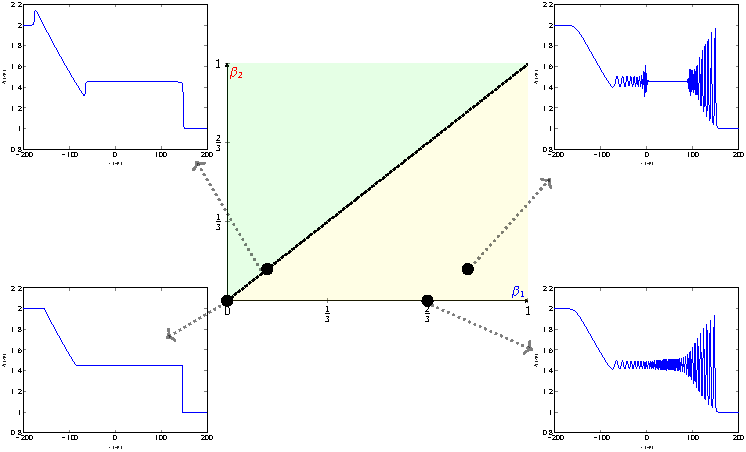
\includegraphics[width=1\textwidth]{3x3Grid.pdf}
	\caption{Example numerical solutions to dam break problem from family of non-linear dispersive water wave model}
\end{figure}
We describe a numerical scheme for solving the generalised Serre-Green-Naghdi equations. This numerical scheme is an extension to the numerical scheme for the classical Serre-Green-Naghdi equations written in conservation law form. This numerical scheme solves an elliptic equation for the non-conservative variable and then evolves the conserved variables through time using the finite volume method. We then describe a typical second-order implementation of this numerical scheme which is validated using known analytic solutions; the travelling solitary wave and the dam-break problem. The numerical method is further validated for general members of this family of equations using forced solutions. The described numerical method is shown to be conservative, robust and second-order accurate.



\end{document} 